\documentclass[10pt]{article}

\usepackage[makeroom]{cancel}
\usepackage{amsfonts,amssymb,fullpage,enumerate,amsmath,color}
\usepackage{subfigure, graphics}
\usepackage{ragged2e}
\usepackage{adjustbox,setspace}
\usepackage[caption=false]{subfig}
\usepackage{color}
\usepackage{url}
\usepackage{minibox}
\usepackage[colorinlistoftodos]{todonotes}
\usepackage[linesnumbered,ruled]{algorithm2e}

% \usepackage[demo]{graphicx}
% \usepackage{subfig}

\DeclareMathOperator*{\argmin}{arg\,min}
\DeclareMathOperator*{\argmax}{arg\,max}

\newcommand{\enc}{\text{Enc}}
\newcommand{\st}{\text{\quad subject to \quad}}

\newcommand{\F}{\mathcal{F}}

\newcommand{\FF}{F}
\newcommand{\GG}{G}

\newcommand{\why}{{\color{red}(why?)}}





\pagestyle{plain}

%------------------------------------------------------------------------------$
\begin{document}

\title{Notes on Wireless Experiments (AOA)}
\maketitle

\section{Fundamentals}

\subsection{sine waves}
Sine wave is the simplest wave form that you can imagine (see first row in Figure~\ref{fig:carrier}).  It oscillates between $-A$ and $A$.  Each point on the wave is represent as $A\cdot \textbf{sin}(\theta)$ where $\theta = \omega t + \phi$ is a function of time $t$.\footnote{Note that representing a point using $A\cdot \textbf{sin}(\theta)$ tells you whether the wave will go up or down in the next instant.}

In many cases, we would represent the tuple $(A, \theta)$ as a single complex number 
\begin{align} 
a + bi = A(\textbf{cos}(\theta)+i\cdot\textbf{sin}(\theta))
\label{eq:complex}
\end{align} 

\subsection{carrier waves}
Carrier wave is just the sine wave.  When we say 2.4GHz or mmWave, we are referring to the frequency of the carrier wave.  The frequency of the carrier wave determines how well the signal can penetrate walls, etc.

The carrier wave is generated by an oscillator in the baseband generator (e.g., usrp).  The generator can adjust the carrier frequency, stop and start sending, and change the phase offset wave easily.  We need antennas with the right spec to send and receive the signal.


\begin{figure}[h!]
\begin{center}
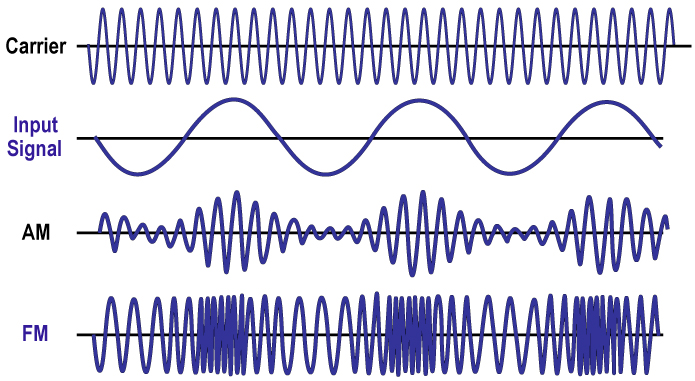
\includegraphics[width=0.6\linewidth]{figs/carrier}
\end{center}
\caption{Carrier wave is the uninteresting wave that does not do anything yet.}
\label{fig:carrier}
\end{figure}



\subsection{modulated waves}
We manipulate the carrier wave to make it carry information.  We can adjust the magnitude (AM, amplitude modulation), the frequency (FM, phase modulation), or the phase of the carrier wave (BPSK, binary phase shift keying).  One can do combinations of these three manipulation methods to create a whole bunch of different modulation methods.

We we encode discrete data, we call each data unit a symbol (in BPSK we encode one bit at a time, in QPSK two bits are encoded each time).  The number of symbols we encode in a given time determines the symbol rate.  Symbol rate times the number of bits per symbol gives us the data throughput.

Note that the modulated wave can still be represented as a sequence of complex numbers.

\begin{figure}[h!]
\begin{center}
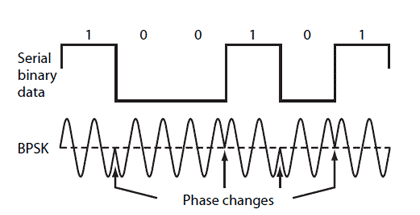
\includegraphics[width=0.6\linewidth]{figs/bpsk}
\end{center}
\caption{Encoding information by changing phase of the carrier wave at the right times.}
\label{fig:bpsk}
\end{figure}


\subsection{measuring wireless signal}
The modulated wave will be modified by the channel after its being transmitted.  There are mainly 3 effects that will happen: (1) the phase will change by $\triangledown\theta=\frac{2\pi d}{T}$ where $d$ is the distance traveled and $T=\frac{1}{f}$, (2) the magnitude will decrease based on the attenuation of the channel\footnote{Attenuation is also related to distance.}, and (3) noise will be added\footnote{If we assume Gaussian noise (AWGN channel, additive white Gaussian noise), then adding noise is just adding a complex number with uniform random phase and zero mean Gaussian magnitude.}.  If there are multiple paths reaching the same antenna, then the result is simply the sum of all signals (i.e., just add all the complex numbers from each path).


Normally, one would measure the effect of channel first by transmitting some know signal, which is called the preamble.  This helps the receiver to measure what the channel does\footnote{Channel estimation is basically trying to solve for $h$ so that $c_{rx} = h\cdot c_{tx}$. }.  Once a signal is received, the receiver will try to reverse the channel affect to get back the modulated signal.  Then the receiver can perform demodulation to recover the embedded information (or symbols).


\section{AOA estimation}

\subsection{Basic Idea}
When there are multiple antennas receiving at the same time, we can estimate the difference in traveling distance from the source to each antenna by looking at the phase of received signals.  Assume that only the line of sight path exists.  Let $d_i$ be the distance from source to antenna $i$, we know that the phase $p_i$ of a complex number received by antenna $i$ would be $\theta + \frac{2\pi d_i}{T}$.  So by subtracting $p_i$ and $p_j$, we have the following constraint:
\begin{align}
&\frac{2\pi d_i-d_ij}{T} = p_i - p_j & \textbf{mod}2\pi\\
\implies& d_i-d_j = \frac{T}{2\pi}(p_i - p_j)  & \textbf{mod}2\pi
\end{align}
In certain settings, knowing the difference in traveled distance can then help us to determine the AOA, as shown in Figure~\ref{fig:aoa}.  In this figure, $d\cdot\textbf{sin}(\theta) = d_i-d_j$.

\begin{figure}[h!]
\begin{center}
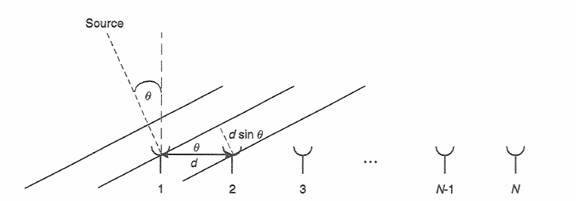
\includegraphics[width=0.6\linewidth]{figs/AOA}
\end{center}
\caption{The phase offset between each antenna reflects the difference in traveled distance, which we can use to estimate the angle of arrival.}
\label{fig:aoa}
\end{figure}

This method shows that angular information can be extracted from samples received from multiple antennas.  Note that in a perfect world, we only need one sample from each antenna to estimate AOA.

\subsection{Correlation Method}
In a world where multi-path and noise exist, the basic method may not work well.  The idea of correlation method is to generate simulated signals for each AOA, and then try to see which one has the best correlation with the received signal.  The set of generated signal are often called the steering vectors.  Each steering vector is a $n\times1$ vector where $n$ is the number of antennas.

When there are two different AOAs from multi-path, one should expect to see two steering vectors that has high correlation with the received signal.

\subsection{Music}
Music is similar to correlation method, but better.  See \textbf{DOA methods.pdf} in the same folder for more information about these algorithms.




\section{Hardware Setup}
\subsection{Antennas}
There are big antennas and small antennas.  The only difference I'm aware of is that the larger ones have stronger signal.  
\subsection{USRP}
USRP is a magical device that generates the carrier wave and does the modulation.  There are two boards in an USRP.  The daughter board, which is attached to the main board, seems to control the carrier frequency range.  The antennas are connected to the daughter board.  In our lab, there are USRPs of frequency range 2.4-6GHz, and ones that are 68.76 MHz to 2.2 GHz.  Most of the working URSPs have the same version of firmware installed.  

Make sure the power is turned off when installing/removing antennas.  Rumors say that the usrp could burn if not handled correctly.



\subsection{DELL}
The Dell machine talks to USRPs through a driver called UHD (USRP Hardware Driver).  It has interfaces in C that lets you control how and what to send and receive.  One dell machine can talk to multiple USRPs.  The Dell machines are connected to the USRPs through ethernet cable with at least 1Gb/s speed.  Note that using usb dongles often reduces the speed, and in those cases USRP will refuse to talk.


\subsection{clock}
One assumption we made earlier is that all receiving antennas are synchronized (i.e., they samples at the exact same time in the exact same frequency).  We use an external clock to synchronize their sampling frequency.  The clock has 
two outputs that need to be connected to the USRP.  

Note that clock only ensures that USRPs sample at the same frequency, but they still might sample at different times which causes an arbitrary phase offset between USRPs.  We calibrate the phase offset by using sending a reference signal that is right in front of the antenna array \footnote{This is not necessarily the right method.  There are fancier hardware that can synchronize both phase and frequency.}.


\section{Software Setup}
\subsection{Tx node}
On Tx node, there is a binary data file generated before hand (e.g. \textbf{ones1000.dat} contains 1000 ones in binary format).  \textbf{aoa\_tx.cpp} reads in the data file and sends it at the selected frequency, gain, and symbol rate.  Gain is normally set to 25 and I have never changed it before.  Lower symbol rate means it will take longer to transmit the same data.

The script \textbf{start\_tx.sh} sends the data file from reference antenna, wait for some time, then send another file through the target antenna.


\subsection{Rx node}
\textbf{4rx\_to\_file.cpp} receives signal at a selected frequency, gain, and symbol rate for a given time.  The file is saved locally in binary format, and contains a sequence of complex numbers.

\textbf{trim\_data.py} scans through the received data file and removes sections where no signal is removed.  This saves a lot of time when transferring the log file.

\subsection{control}
The controlling computer runs \textbf{start\_exp.sh}, which runs the entire experiment and move the log file locally for display.



\end{document}
